% Chapter Template

\chapter{Efficacy Transition Pathways} % Main chapter title

\label{etp} % For referencing this chapter elsewhere, use \ref{etp}

%----------------------------------------------------------------------------------------
%	SECTION 1
%----------------------------------------------------------------------------------------

\section{Introduction}
\label{etp:Introduction}

Phase \RN{2} trials build upon the work of early Phase \RN{1} trials where preliminary information is obtained regarding the safety profile and dose schedule of a treatment. The key output from a Phase \RN{1} trial is the MTD (Maximum Tolerated Dose), TD\%\% (target dose at some pre-specified level), RP2D (Recommended Phase \RN{2} Dose) or OBD (optimal biological dose) i.e. some dose-level that can be taken forward for future testing. In Phase \RN{2} trials the focus shifts away from toxicity and looks more towards efficacy of these new treatments at the dose-levels previously defined \cite{berryBayesianAdaptiveMethods2010}. The purpose of phase \RN{2} trials is to usually see if a new treatment or intervention works and establish if there is a efficacy signal. More specifically they aim to determine if there is a sufficient level of efficacy to warrant further research in for example a Phase \RN{3} setting \cite{juliousIntroductionStatisticsEarly2010}. In addition to assessing efficacy there is also opportunity to further explore the toxicity profile of the treatment as in comparison to Phase \RN{1} trials Phase \RN{2} trials are typically conducted using a larger sample size.  

Phase \RN{2} trials can be categorised further, dependent on the primary aims of the trial. Single-arm trials can be classified as Phase \RN{2} A trials, here a sample of patients would be given the experimental treatment and efficacy would be assessed. There are also multi-arm trials which may randomise patients to multiple experimental treatments or between an experimental treatment and standard of care. Efficacy would then be compared across the different arms. These types of trials are commonly referred to as Phase \RN{2} B trials. 

Generally speaking Phase \RN{2} trials should be efficient and quick such that we can progress to Phase \RN{3} as quickly as possible or drop any ineffective treatments. The output from a Phase \RN{2} trial should be either a 'GO' or 'No GO' decision i.e should we or should we not proceed to later phase testing based on the data observed in this trial. One of the more important aspects of these trials is that we don't want to make any incorrect decisions and if there is an effective treatment that is being investigated we want to make sure that it is taken forward into Phase \RN{3}.

An example of a Phase II single arm trial design is depicted in Figure \ref{fig_etp:phase2_singlearm_example}. For single-arm Phase \RN{2} trials eligible patients come into the trial and all of them will be allocated to the new treatment. Once they have completed their treatment period we would then assess the effectiveness of that treatment using some measure of success. Looking at the outcome of success in each patient the success rate or proportion of success can then be determined. In the single arm setting, this success rate is then compared to some sort of benchmark, which is determined from either historical data or clinical input.


\begin{figure}[h!]
	\centering
	\caption{Example of a Phase 2 single arm trial design.}
	\label{fig_etp:phase2_singlearm_example}
	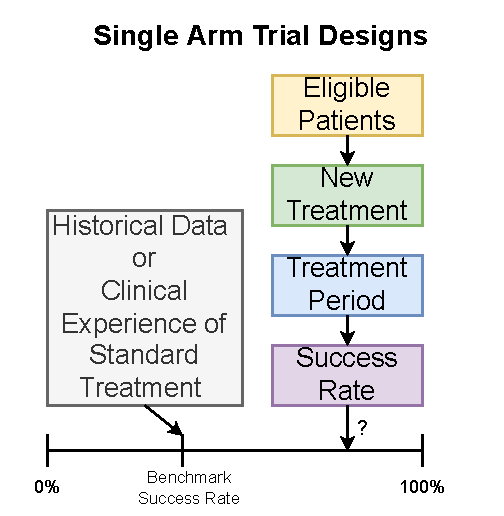
\includegraphics[width=0.75\textwidth]{ETP-Phase2SingleArmExample}
\end{figure}

The primary outcome measure for a trial like this should be some short-term binary outcome either success or failure. The outcome measure selected should be chosen such that you expect the treatment to have an effect on that. Typically these are surrogates for longer-term efficacy measures. So, if we see a success in the Phase II trial we would hope there would also be some long-term benefits for patients as well. In the oncology setting Phase III trials typically will look at outcomes such as survival times but in the previous Phase II trials response or change in tumour size may have been used as outcomes.

There are many classical frequentist approaches which can be applied to Phase \RN{2} trials such as the Flemming A'Hern, Simons two-stage or Bryant and Day designs. However, there exist complex and innovative designs that are adaptive in nature and allow for more frequent interim analyses so decisions can be made faster. 

One approach is Bayesian and utilises a Beta-Binomial conjugate analysis to estimate a  response rate for a binary outcome. Posterior probabilities can be used to inform decision making and predictive probabilities can be used during interim analyses in a similar manner. This is typically done using pre-specified decision rules.

Whilst mathematically simple to implement a design such as this has similar drawbacks to dose-finding methodologies that have been previously discussed. Due to its flexibility there may be some issues with parametrising the design, in this case would mean selecting the correct decision rules. A Bayesian approach may be less familiar than traditional frequentist approaches that are more commonly used. It may also be hard to understand why certain decisions are being made during interim and final analyses.  

One potential solution to these problems was devised by Lucinda Billingham who developed Efficacy Transition Pathways (ETPs) a novel visualisation tool to aid the design and interpretation of these types of trial designs. ETPs extend on the idea of dose transition pathways, which solves for many of the same issues in dose-finding trials. 

In this chapter we will explore the components that go into constructing an ETP for a Beta-Binomial conjugate analysis. We will detail how ETPs can be used in a trial setting with an illustrative example. Finally, we also provide details on a web application that can be used to produce ETPs and acts as an educational tool to explain what they are. 

%----------------------------------------------------------------------------------------
%	SECTION 2
%----------------------------------------------------------------------------------------

\section{Beta-Binomial Conjugate Analyses}

Bayesian methods are an alternative way of thinking about evidence, data and statistics compared to the traditional frequentist approach. The Bayesian approach could be considered more intuitive and has some advantages that make it useful for analysing clinical trials. 

The fundamentals of Bayesian statistics are well defined in the literature as well as its application to clinical trials and health research. Bland and Altman \cite{blandBayesiansFrequentists1998} discuss the differences between a Bayesian or a frequentist approach. Spiegelhalter et al. \cite{spiegelhalterIntroductionBayesianMethods1999} detail the underlying philosophy behind Bayesian methods along with its application in health technology assessment. General Bayesian methods are described in more detail in books by Lee \cite{leeBayesianStatisticsIntroduction2012} and Bernado and Smith \cite{bernardoBayesianTheory2009}. It should be noted, these are just a few examples from the literature.    

The Bayesian paradigm doesn’t regard parameters, things we don’t know like a treatment effect ($\theta$), as fixed. These are instead thought of to be uncertain. Bayesian statistics uses probability to express this uncertainty. Since $\theta$ is unknown, it has a probability distribution. 

Bayesian analysis takes into account prior information on $\theta$ which also has the form of a probability distribution. This is combined with the likelihood of the data, Y given $\theta$, to produce a posterior probability distribution of $\theta$ given Y. So, data is collected to find out about the parameter. This data can be regarded as known and fixed and is used to estimate the unknown parameter. In Bayesian statistics, we estimate the probability of the parameter given the data.

Once a posterior distribution is established inferences can then be made about $\theta$. However, this may require numerical integration of the posterior distribution which may be difficult or impossible to evaluate analytically. An option around this is to use conjugate priors. If the posterior distribution and the prior distribution are from the same probability distribution family these can be referred to as conjugate distributions and the prior as a conjugate prior. Conjugate priors are algebraically easier to deal with and allow for easier interpretation of the posterior distribution. 

One example of this is what is commonly referred to as the Beta-Binomial conjugate. This is where the prior and posterior distributions take the form of a Beta distribution and the likelihood or data is Binomial. 

Binomial data has two possible outcomes. For example, a coin toss has two outcomes either its head or its tails. In the context of a Phase II single arm trial, this could be either a success/failure to some new treatment or response/no response. When this is combined with a Beta prior distribution we get a posterior Beta distribution. From this, we can then make probability statements about the treatment effect.

Following the explanation by Lee \cite{leeBayesianStatisticsIntroduction2012} of a Beta conjugate prior for a binomial distribution. Consider a parameter of interest $\theta$ that represents some treatment effect. More specifically, for binomial data in a single arm Phase \RN{2} clinical trial, lets say the parameter $\theta$ is the probability of response in a number of patients following a some new treatment. Each patient can experience either a response or no response, with the same probability of response and each patient being independent from each other. For a fixed sample size with $n$ patients and number of responses ($y$) we have: 

\begin{equation}
	y \sim \text{Binomial}(n, \theta)
\end{equation}

So, $y$ is from a binomial distribution which produces the following likelihood: 

\begin{equation}
	L(\theta) = P(y|\theta) = {n \choose y}\theta^y (1-\theta)^{n-y} \; \; \; \; (y = 0,1,\ldots,n)
\end{equation}

If the prior for $\theta$ is from a Beta distribution such that 

\begin{equation}
	P(\theta) = \text{Beta}(a,b)
\end{equation}

then the posterior distribution is also from a Beta distribution and can be expressed as 

\begin{equation}
	P(\theta|y) = \text{Beta}(a+y,b+n-y)
\end{equation}

Using the posterior distribution for $\theta$ we can go on to make summary estimates and interpret the treatment effect. 
%-----------------------------------
%	SUBSECTION 1
%-----------------------------------

\subsection{Interim analyses and Predictive Probability of Success}

%----------------------------------------------------------------------------------------
%	SECTION 3
%----------------------------------------------------------------------------------------

\section{Constructing Efficacy Transition Pathways}

%-----------------------------------
%	SUBSECTION 1
%-----------------------------------

\subsection{Illustrative example using the DETERMINE trial}

%----------------------------------------------------------------------------------------
%	SECTION 4
%----------------------------------------------------------------------------------------

\section{Development of a Web Application for ETPs}